\documentclass [12pt]{georeport}

\newcommand{\du}{\delta u}
\newcommand{\dm}{\delta m}
\newcommand{\lu}{\lambda u}
\newcommand{\lm}{\lambda m}
\newcommand{\muu}{\mu u}
\newcommand{\bF}{{\bf F}}
\newcommand{\bS}{{\bf S}}
\newcommand{\bH}{{\bf H}}
\newcommand{\bM}{{\bf M}}
\newcommand{\bR}{{\bf R}}
\newcommand{\bu}{{\bf u}}
\newcommand{\bx}{{\bf x}}
\newcommand{\bv}{{\bf v}}
\newcommand{\be}{{\bf e}}
\newcommand{\bp}{{\bf p}}
\newcommand{\cS}{{\cal S}}

\newcommand{\peq}{\,+\hspace{-0.15cm}=}
\newcommand{\pp}{\,+\hspace{-0.1cm}+}
\newcommand{\mm}{\,-\hspace{-0.1cm}-}


\begin{document}
\title{IWAVE Demonstration Package - Draft 22.08.12}
\author{William. W. Symes \thanks{The Rice Inversion Project,
Department of Computational and Applied Mathematics, Rice University,
Houston TX 77251-1892 USA, email {\tt symes@caam.rice.edu}.}}

\maketitle
\parskip 12pt
\begin{abstract}
IWAVE is a framework for time-domain regular grid finite difference and finite element methods. The demonstration package includes examples of typical IWAVE use cases, with complete input data. This paper displays reference output. [Note - under construction!]
\end{abstract}

\section{Introduction}
The primary purpose of this short paper is to illustrate the use of IWAVE to calculate synthetic seismograms. IWAVE is built around a core framework, that is, a collection of separate software packages which together provide a set of essential services upon which applications may be built, and which completely define the interfaces to which additional software must be written to formulate a complete application. Along with the core framework, the current release contains a complete time-domain acoustic modeling application, as well as a basic isotropic elastodynamics application.
The demonstrations discussed here are based on the acoustic modeling application.

All IWAVE applications are parameter-driven: that is, they accept as input a file defining a {\em map} or associative array, consisting of a list of {\tt key = value} pairs. The demo directories described in this paper contain one or more such parameter (``par'') files, always signified by the suffix ``{\tt .par}''. Each file defines a modeling task. By perusing these par files and examining the simulation output, the user can quickly gain an appreciation of scope of IWAVE's capabilities. 

A secondary purpose is to supply the user with the means to independently verify some of the claims in the paper by \cite{SymesVdovina:09}, in which the examples were generated using an earlier version of the same software.

\section{Acoustodynamics}
The IWAVE acoustic package is based on the pressure-velocity form of acoustodynamics, consisting of two coupled first-order partial differential equations:
\begin{eqnarray}
\label{awe}
\rho \frac{\partial \bv}{\partial t} &=& - \nabla p \\
\frac{1}{\kappa}\frac{\partial p}{\partial t} &=& -\nabla \cdot \bv + g
\end{eqnarray}
In these equations, $p(\bx,t)$ is the pressure (excess, relative to an ambient equilibrium pressure), $\bv(\bx,t)$ is the particle velocity, $\rho(\bx)$ and $\kappa(\bx)$ are the density and particle velocity respectively. Bold-faced symbols denote vectors; the above formulation applies in 1, 2, or 3D. 

The inhomogeneous term $g$ represents externally supplied energy (a
``source''), via a defect in the acoustic constitutive relation. A
typical example is the {\em isotropic point source}
\[
g(\bx,t) = w(t) \delta(\bx-\bx_s)
\]
at source location $\bx_s$.

The bulk modulus and buoyancy (reciprocal density) are the natural parameters in a time-stepping discretization of this equation. I will display velocity and density instead. IWAVE's acoustic application converts velocity and density to bulk modulus and buoyancy as part of the problem setup phase.

\section{The dome model}

This simple 2D model embeds an anticline or dome in an otherwise
undisturbed package of layers. The velocity and density models are
depicted in Figures \ref{fig1} and \ref{fig2}.

\cite[]{SymesVdovina:09} use this model to illustrate the {\em
  interface error} phenomenon: the tendency, first reported by
\cite[]{Brown:84}, of all finite difference schemes for wave
propagation to exhibit first order error, regardless of formal order,
for models with material parameter discontinuities. The shot record
(Figure \ref{fig3}, acquisition geometry described in caption) looks
perfectly normal. However the spatial sample rate of the model in
Figures \ref{fig1} and \ref{fig2} has a considerable effect. The
material parameter fields are constructed as {\em functions} of
position in 2D space, hence can be sampled at any rate at all. Figures
\ref{fig4} and \ref{fig5} compare traces computed from models sampled
at four different rates. The scheme used is the 2nd order in time,
4th order in space staggered grid scheme, which is formally 2nd order
convergent like the original 2nd order scheme suggested by
\cite[]{Vir:84}, but has better dispersion suppression. Nonetheless,
the figures clearly show the first order error, in the form of a
grid-dependent time shift, predicted by \cite[]{Brown:84}. See
\cite{SymesVdovina:09} for more examples, analysis, and discussion.

\section{Building IWAVE outside of Madagascar}
IWAVE and all of its parts build with SConstruct, either as part of the Madagascar environment, or independently. This section describes the build of the IWAVE demos in a standalone installation. 

For instructions on TRIP software (including IWAVE) independently of Madagascar, see 
\begin{verbatim}
www.trip.caam.rice.edu/software/admin/doc/html/install.html
\end{verbatim}

To build the IWAVE demo examples and this pdf document,
\begin{itemize}
\item install IWAVE somewhere, following the instructions in the web document referenced above - I will use  {\tt \$IWAVE} to denote
  the path to the top-level IWAVE directory;  
\item build {\tt demo1}, {\tt demo2},...:
\begin{itemize}
\item {\tt cd \$IWAVE/demo/demo1}
\item {\tt scons}
\end{itemize}
\item install the figures (this is optional, only needed if you have done something to change them - reference figure files are included with the download)
\begin{itemize}
\item {\tt cd \$IWAVE/demo/demo1/fig}
\item {\tt cp fig*.ps ../../Fig}
\end{itemize}
\item build this document:
\begin{itemize}
\item {\tt cd \$IWAVE/demo}
\item {\tt scons}
\end{itemize}
\end{itemize}
Note that the finest (2.5 m) grid used in any of the {\tt demo1} examples consists of roughly 10 million
gridpoints. Consequently the modeling runs collectively take a few
minutes on a single thread, for this example. The coarsest grid (20 m) on the other hand runs in a couple of seconds. 

It is possible to run individual examples within each demo directory: for example,
\begin{verbatim}
cd $IWAVE/demo/demo1
scons demo20m
\end{verbatim}
will produce a directory {\tt \$IWAVE/demo/demo1/demo20m}, within which you will 
find all of the result files for this example, always including the output data file {\tt data.su}.

Inspection of the {\tt SConstruct} file in {\tt demo1} will show that
the modeling tool used is {\tt \$IWAVE/asg2/main/asg.x}, the IWAVE
acoustic modeling command. This command reads its parameters from a
par file. Four par files are present in {\tt demo1}, each one defining
a modeling job, corresponding to a given level of grid refinement. The
meaning of each parameter in the par file is described in the IWAVE
web documentation:
\begin{verbatim}
www.trip.caam.rice.edu/software/iwave/doc/html/index.html
\end{verbatim}
All other demos are organized similarly.

\section{Acknowledgements}
Development of IWAVE was supported by the SEG Advanced Modeling (SEAM) project, by the National Science Foundation under awards 0620821 and 0714193, and by the sponsors of The Rice Inversion Project. The IWAVE project owes a great deal to several open source seismic software packages (Seismic Un*x, SEPlib, Madagascar), debts which we gratefully acknowledge. 
\bibliographystyle{seg}
\bibliography{masterref}

\newpage

\begin{figure}
\label{fig1}
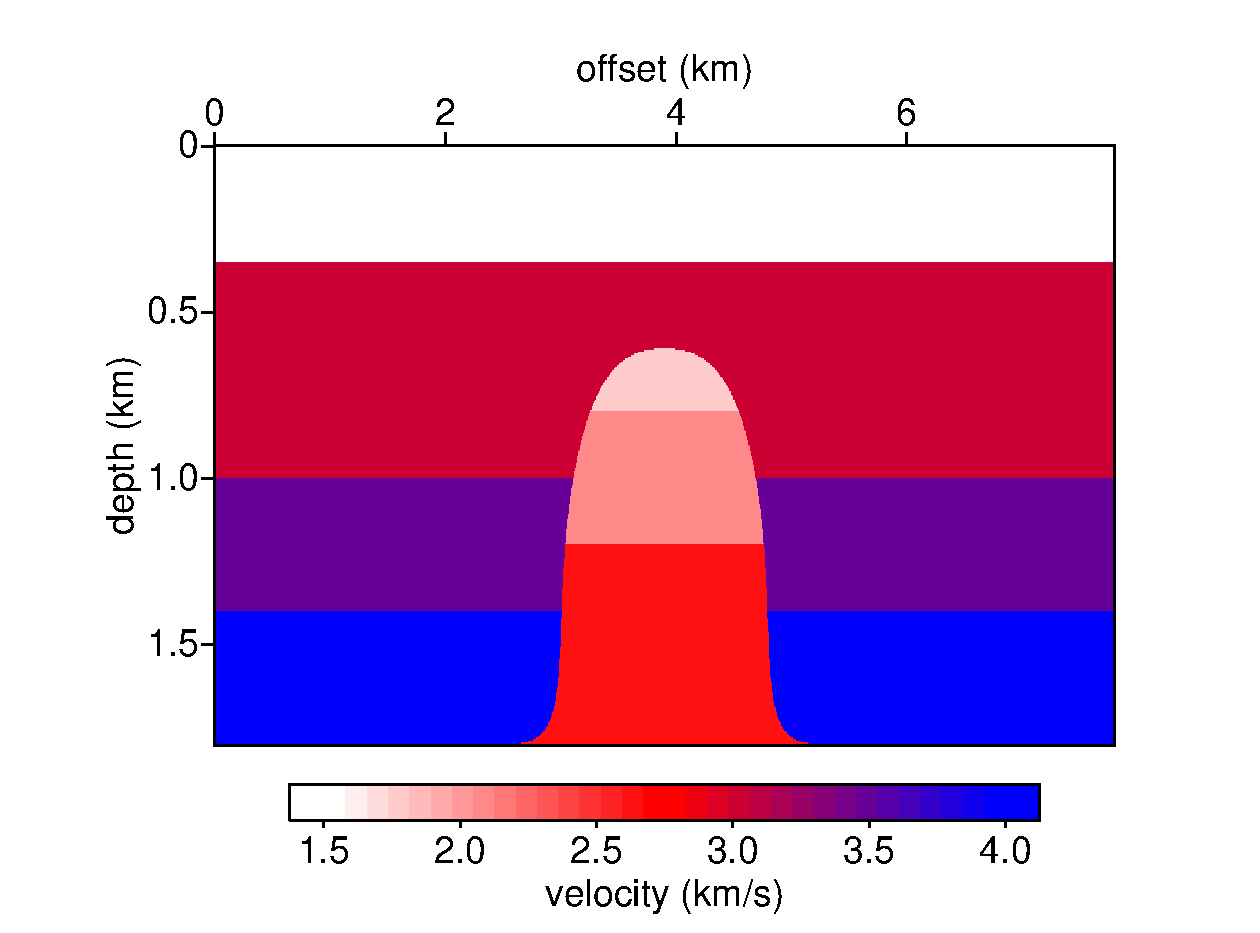
\includegraphics[height=10cm,width=15cm]{./Fig/fig1.ps}
\caption{Dome velocity model}
\end{figure}

\begin{figure}
\label{fig2}
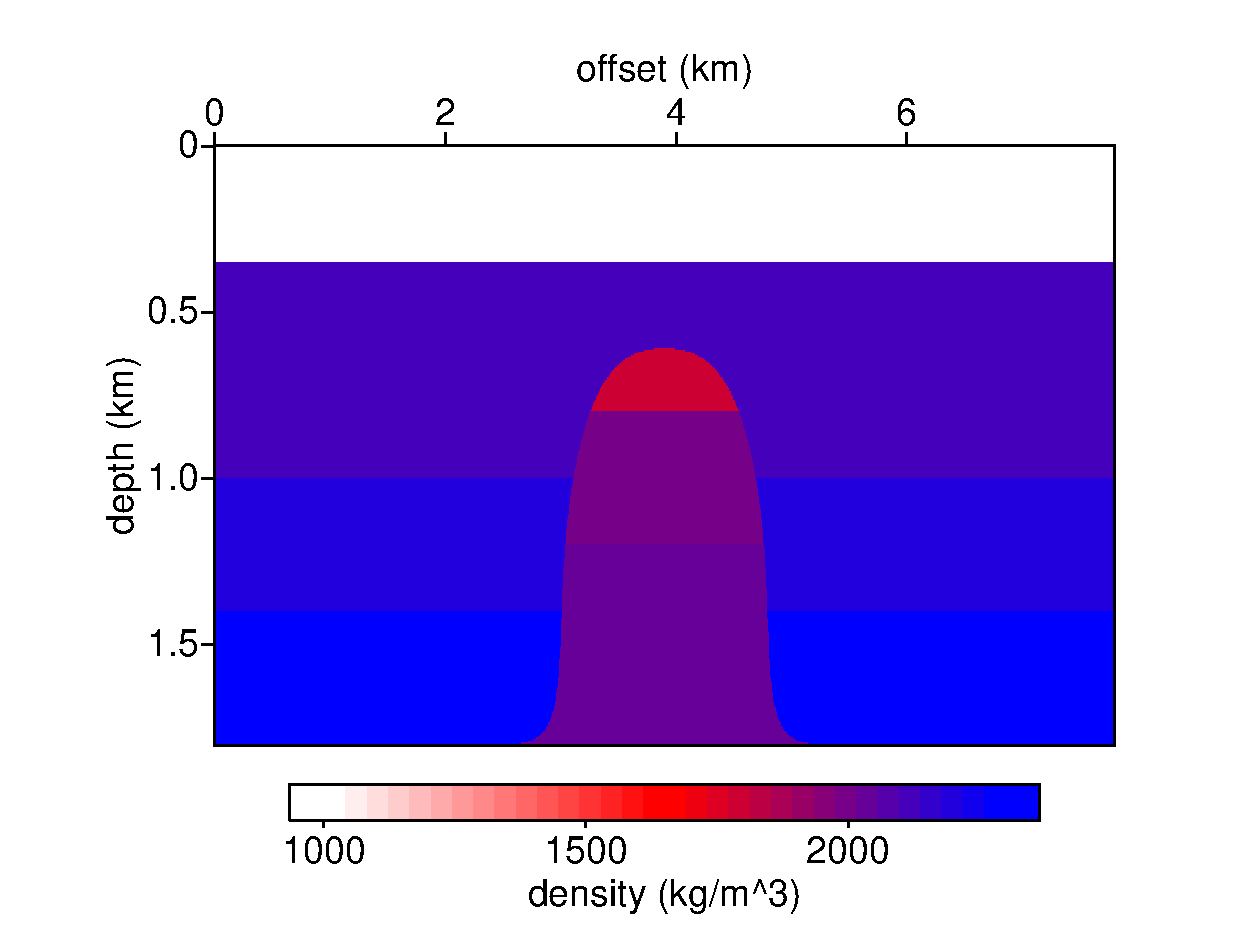
\includegraphics[height=10cm,width=15cm]{./Fig/fig2.ps}
\caption{Dome density model}
\end{figure}

\begin{figure}
\label{fig3}
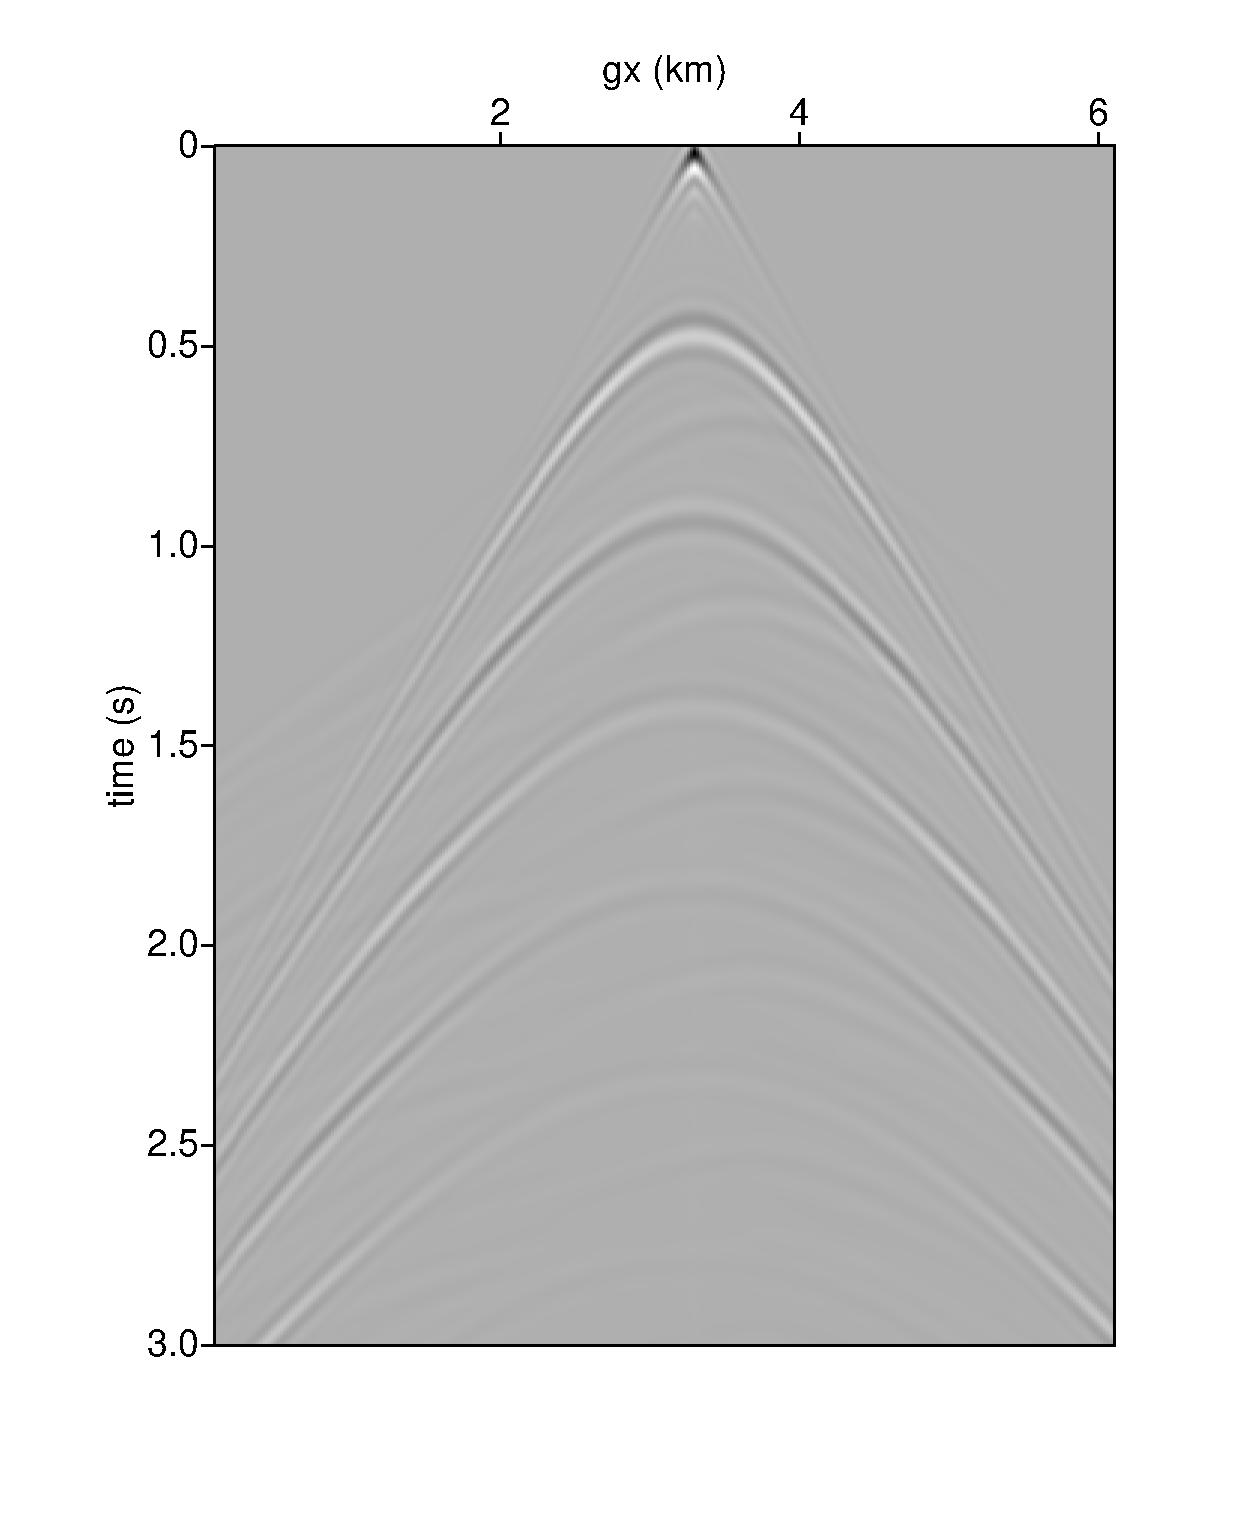
\includegraphics[height=15cm,width=15cm]{./Fig/fig3.ps}
\caption{2D shot record, 301 traces: shot x = 3300 m, shot z = 40 m, receiver x =
  100 - 6100 m, receiver z = 20 m, number of time samples = 1501, time
sample interval = 2 ms. Source pulse = zero phase trapezoidal [0.0,
2.4, 15.0, 20.0] Hz bandpass filter. }
\end{figure}

\begin{figure}
\label{fig4}
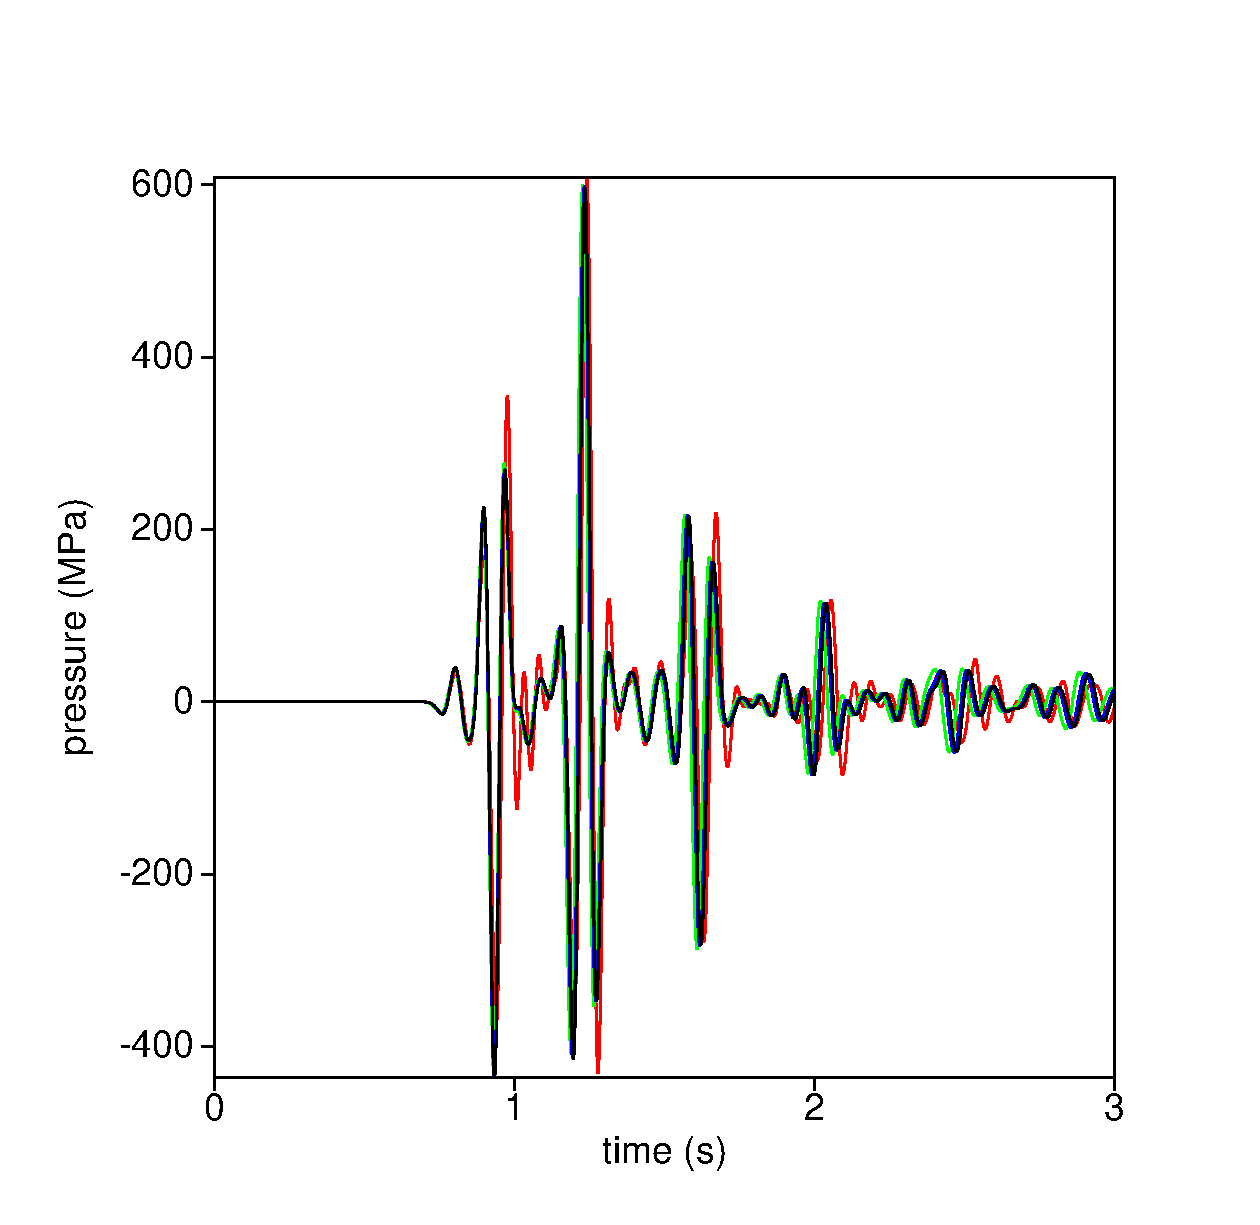
\includegraphics[height=15cm,width=15cm]{./Fig/fig4.ps}
\caption{Trace 100 (receiver x = 2100 m) for $\Delta x = \Delta z = $
  20 m (red), 10 m (green), 5 m (blue), and 2.5 m (black). Note
  arrival time discrepancy after 1 s: this is the interface error
  discussed in \cite{SymesVdovina:09}. Except for the 20 m result,
  grid dispersion error is minimal.} 
\end{figure}

\begin{figure}
\label{fig5}
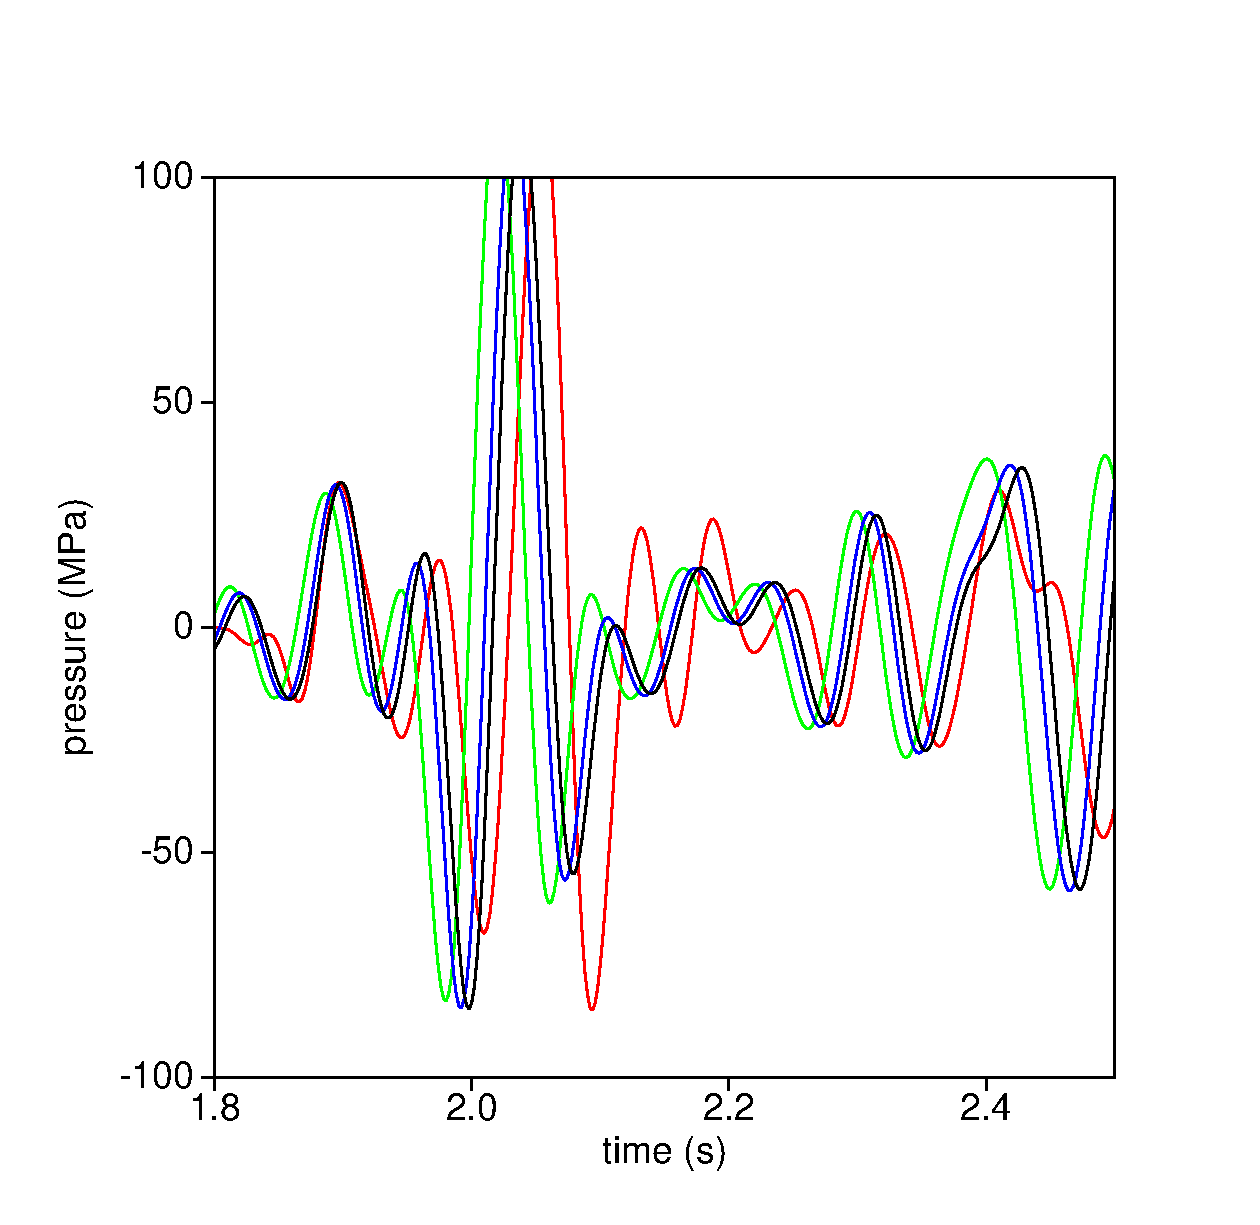
\includegraphics[height=15cm,width=15cm]{./Fig/fig5.ps}
\caption{Trace 100 detail, 1.8-2.5 s, showing more clearly the
  first-order interface error: the time shift between computed events
  and the truth (the 2.5 m result, more or less) is proportional to
  $\Delta t$, or equivalently to $\Delta z$.}
\end{figure}

\end{document}

